
%% bare_conf.tex
%% V1.3
%% 2007/01/11
%% by Michael Shell
%% See:
%% http://www.michaelshell.org/
%% for current contact information.
%%
%% This is a skeleton file demonstrating the use of IEEEtran.cls
%% (requires IEEEtran.cls version 1.7 or later) with an IEEE conference paper.
%%
%% Support sites:
%% http://www.michaelshell.org/tex/ieeetran/
%% http://www.ctan.org/tex-archive/macros/latex/contrib/IEEEtran/
%% and
%% http://www.ieee.org/

%%*************************************************************************
%% Legal Notice:
%% This code is offered as-is without any warranty either expressed or
%% implied; without even the implied warranty of MERCHANTABILITY or
%% FITNESS FOR A PARTICULAR PURPOSE! 
%% User assumes all risk.
%% In no event shall IEEE or any contributor to this code be liable for
%% any damages or losses, including, but not limited to, incidental,
%% consequential, or any other damages, resulting from the use or misuse
%% of any information contained here.
%%
%% All comments are the opinions of their respective authors and are not
%% necessarily endorsed by the IEEE.
%%
%% This work is distributed under the LaTeX Project Public License (LPPL)
%% ( http://www.latex-project.org/ ) version 1.3, and may be freely used,
%% distributed and modified. A copy of the LPPL, version 1.3, is included
%% in the base LaTeX documentation of all distributions of LaTeX released
%% 2003/12/01 or later.
%% Retain all contribution notices and credits.
%% ** Modified files should be clearly indicated as such, including  **
%% ** renaming them and changing author support contact information. **
%%
%% File list of work: IEEEtran.cls, IEEEtran_HOWTO.pdf, bare_adv.tex,
%%                    bare_conf.tex, bare_jrnl.tex, bare_jrnl_compsoc.tex
%%*************************************************************************

% *** Authors should verify (and, if needed, correct) their LaTeX system  ***
% *** with the testflow diagnostic prior to trusting their LaTeX platform ***
% *** with production work. IEEE's font choices can trigger bugs that do  ***
% *** not appear when using other class files.                            ***
% The testflow support page is at:
% http://www.michaelshell.org/tex/testflow/



% Note that the a4paper option is mainly intended so that authors in
% countries using A4 can easily print to A4 and see how their papers will
% look in print - the typesetting of the document will not typically be
% affected with changes in paper size (but the bottom and side margins will).
% Use the testflow package mentioned above to verify correct handling of
% both paper sizes by the user's LaTeX system.
%
% Also note that the "draftcls" or "draftclsnofoot", not "draft", option
% should be used if it is desired that the figures are to be displayed in
% draft mode.
%
\documentclass[conference]{IEEEtran}
% Add the compsoc option for Computer Society conferences.
%
% If IEEEtran.cls has not been installed into the LaTeX system files,
% manually specify the path to it like:
% \documentclass[conference]{../sty/IEEEtran}

% Some very useful LaTeX packages include:
% (uncomment the ones you want to load)


% *** MISC UTILITY PACKAGES ***
%
%\usepackage{ifpdf}
% Heiko Oberdiek's ifpdf.sty is very useful if you need conditional
% compilation based on whether the output is pdf or dvi.
% usage:
% \ifpdf
%   % pdf code
% \else
%   % dvi code
% \fi
% The latest version of ifpdf.sty can be obtained from:
% http://www.ctan.org/tex-archive/macros/latex/contrib/oberdiek/
% Also, note that IEEEtran.cls V1.7 and later provides a builtin
% \ifCLASSINFOpdf conditional that works the same way.
% When switching from latex to pdflatex and vice-versa, the compiler may
% have to be run twice to clear warning/error messages.



% *** CITATION PACKAGES ***
%
%\usepackage{cite}
% cite.sty was written by Donald Arseneau
% V1.6 and later of IEEEtran pre-defines the format of the cite.sty package
% \cite{} output to follow that of IEEE. Loading the cite package will
% result in citation numbers being automatically sorted and properly
% "compressed/ranged". e.g., [1], [9], [2], [7], [5], [6] without using
% cite.sty will become [1], [2], [5]--[7], [9] using cite.sty. cite.sty's
% \cite will automatically add leading space, if needed. Use cite.sty's
% noadjust option (cite.sty V3.8 and later) if you want to turn this off.
% cite.sty is already installed on most LaTeX systems. Be sure and use
% version 4.0 (2003-05-27) and later if using hyperref.sty. cite.sty does
% not currently provide for hyperlinked citations.
% The latest version can be obtained at:
% http://www.ctan.org/tex-archive/macros/latex/contrib/cite/
% The documentation is contained in the cite.sty file itself.



% *** GRAPHICS RELATED PACKAGES ***
%
\ifCLASSINFOpdf
   \usepackage[pdftex]{graphicx}
  % declare the path(s) where your graphic files are
   \graphicspath{{../figures/}}
  % and their extensions so you won't have to specify these with
  % every instance of \includegraphics
   \DeclareGraphicsExtensions{.pdf,.jpeg,.png}
\else
  % or other class option (dvipsone, dvipdf, if not using dvips). graphicx
  % will default to the driver specified in the system graphics.cfg if no
  % driver is specified.
  % \usepackage[dvips]{graphicx}
  % declare the path(s) where your graphic files are
  % \graphicspath{{../eps/}}
  % and their extensions so you won't have to specify these with
  % every instance of \includegraphics
  % \DeclareGraphicsExtensions{.eps}
\fi
% graphicx was written by David Carlisle and Sebastian Rahtz. It is
% required if you want graphics, photos, etc. graphicx.sty is already
% installed on most LaTeX systems. The latest version and documentation can
% be obtained at: 
% http://www.ctan.org/tex-archive/macros/latex/required/graphics/
% Another good source of documentation is "Using Imported Graphics in
% LaTeX2e" by Keith Reckdahl which can be found as epslatex.ps or
% epslatex.pdf at: http://www.ctan.org/tex-archive/info/
%
% latex, and pdflatex in dvi mode, support graphics in encapsulated
% postscript (.eps) format. pdflatex in pdf mode supports graphics
% in .pdf, .jpeg, .png and .mps (metapost) formats. Users should ensure
% that all non-photo figures use a vector format (.eps, .pdf, .mps) and
% not a bitmapped formats (.jpeg, .png). IEEE frowns on bitmapped formats
% which can result in "jaggedy"/blurry rendering of lines and letters as
% well as large increases in file sizes.
%
% You can find documentation about the pdfTeX application at:
% http://www.tug.org/applications/pdftex





% correct bad hyphenation here
\hyphenation{op-tical net-works semi-conduc-tor}
% for inline code
\usepackage{courier}
% for block code 
\usepackage{listings}
\lstset{columns=fullflexible,
        mathescape=true,
        literate=
               {=}{$\leftarrow{}$}{1}
               {==}{$={}$}{1},
        morekeywords={if,then,else,return,sqrt}
        }
        

\begin{document}

%
% paper title
% can use linebreaks \\ within to get better formatting as desired
\title{Serendipitous Offline Learning in a Neuromorphic Robot}



% for over three affiliations, or if they all won't fit within the width
% of the page, use this alternative format:
% 
\author{\IEEEauthorblockN{Terrence C. Stewart\IEEEauthorrefmark{1},
Ashley Kleinhans\IEEEauthorrefmark{2},
Andrew Mundy\IEEEauthorrefmark{3} and
J{\"o}rg Conradt\IEEEauthorrefmark{4}}
\IEEEauthorblockA{\IEEEauthorrefmark{1}Centre for Theoretical Neuroscience, University of Waterloo, Waterloo, ON, Canada\\tcstewar@uwaterloo.ca}
\IEEEauthorblockA{\IEEEauthorrefmark{2}Council of Scientific and Industrial Research, Pretoria, South Africa\\akleinhans@csir.co.za}
\IEEEauthorblockA{\IEEEauthorrefmark{3}TODO: Address\\Email}
\IEEEauthorblockA{\IEEEauthorrefmark{4}TODO: Address\\Email}}


% make the title area
\maketitle


\begin{abstract}
%\boldmath
We demonstrate a neuromorphic learning paradigm that is well-suited to embodied learning of complex sensorimotor mappings. A mobile robot is first controlled by a basic set of reflexive hand-designed behaviours. All sensor data is provided via a spike-based silicon retina camera (eDVS), and all control is implemented via spiking neurons simulated on neuromorphic hardware (SpiNNaker). Given this initial control system, the robot is capable of simple obstacle avoidance and random exploration. To train the robot to perform more complex tasks, we observe the robot and find instances where the robot accidentally performs the action we wish it to perform. Data recorded from the robot during these times is then used to update the neural control system, increasing the likelihood of the robot performing that task in the future, given a similar sensor state. We demonstrate this learning approach is sufficient for the robot to learn to turn left or right depending on novel sensory stimuli.

\end{abstract}
% IEEEtran.cls defaults to using nonbold math in the Abstract.
% This preserves the distinction between vectors and scalars. However,
% if the conference you are submitting to favors bold math in the abstract,
% then you can use LaTeX's standard command \boldmath at the very start
% of the abstract to achieve this. Many IEEE journals/conferences frown on
% math in the abstract anyway.
\medskip
\noindent \textbf{Keywords.} adaptive systems, mobile robotics, neurocontrollers, neuromorphics, robot control


\IEEEpeerreviewmaketitle


\section{Introduction}

[CHECK: represent related work and compare them with the proposed approach]

A long-standing dream for robotics is to provide the same sort of
intelligent, adaptive, and flexible behavior that is seen in living
biological systems.  Furthermore, by creating systems that emulate
biological adaptivity, we can investidate intelligence in a very broad sense,
including capabilities that are not yet seen in current machine learning
methods \cite{mcfarland1993intelligent}.  However, it is still a very open
question as to how best to make use of this biological inspiration to construct
improved methods of robotic control.  There are few examples of neural networks 
being used for control \cite{janglova2005neural} in a robotic domain. 
Typically, the hardware used is standard general-purpose computing, and the 
algorithms are machine-learning based. This means that, while they may take
some high-level inspiration from biology, the algorithms themselves do not
directly map to biological details.

Over the last few years, a bridge has been forming between neuroscience and 
robotics \cite{webb2000does}. Ongoing developments in neuromorphic hardware 
design now provide novel computing resources that are more suitable to
directly implementing the types of computations found in biological systems, 
thus facilitating the use of observations and data provided by the 
neuroscience community. Practically speaking, we can now implement large numbers of 
neurons on a very small power budget, making neural control a promising 
energy-efficient direction for mobile robot applications.  Ideally, this could
lead to flexible adaptive control of systems while staying within a limited
power budget.

Our study looks to demonstrate such a flexible control system using 
neuromorphic hardware and neural-based adaptive control. The approach 
combines the SpiNNaker computing 
platform \cite{furber2007neural, furber2014spinnaker}, the Neural Engineering 
Framework (NEF)  \cite{eliasmith2004neural}, and a series of robots developed at 
the Technische Universit{\"a}t M{\"u}nchen. 


For energy efficient implementation given the hardware, the neurn model
employed here is the standard \textit{leaky integrate and fire} (LIF) model, 
where the weighted ($\omega$) sum of input current $I$ causes the voltage $V$ to build up until some
threshold is reached, at which time the neuron emits a discrete spike:

\begin{equation}
    \tau_m {dV \over dt} = -V + \sum \omega I
\end{equation}

When this spike occurs, this causes post-synaptic current to flow into the 
neurons it is connected to, with each connection having its own weight $\omega$
and with the post-synaptic current $h(t)$ exponentially decaying over time, 
as shown in \figurename~\ref{Neuron}:

\begin{equation}
    h(t) = e^{-t/\tau_s}
\end{equation}

\begin{figure}[!t]
\centering
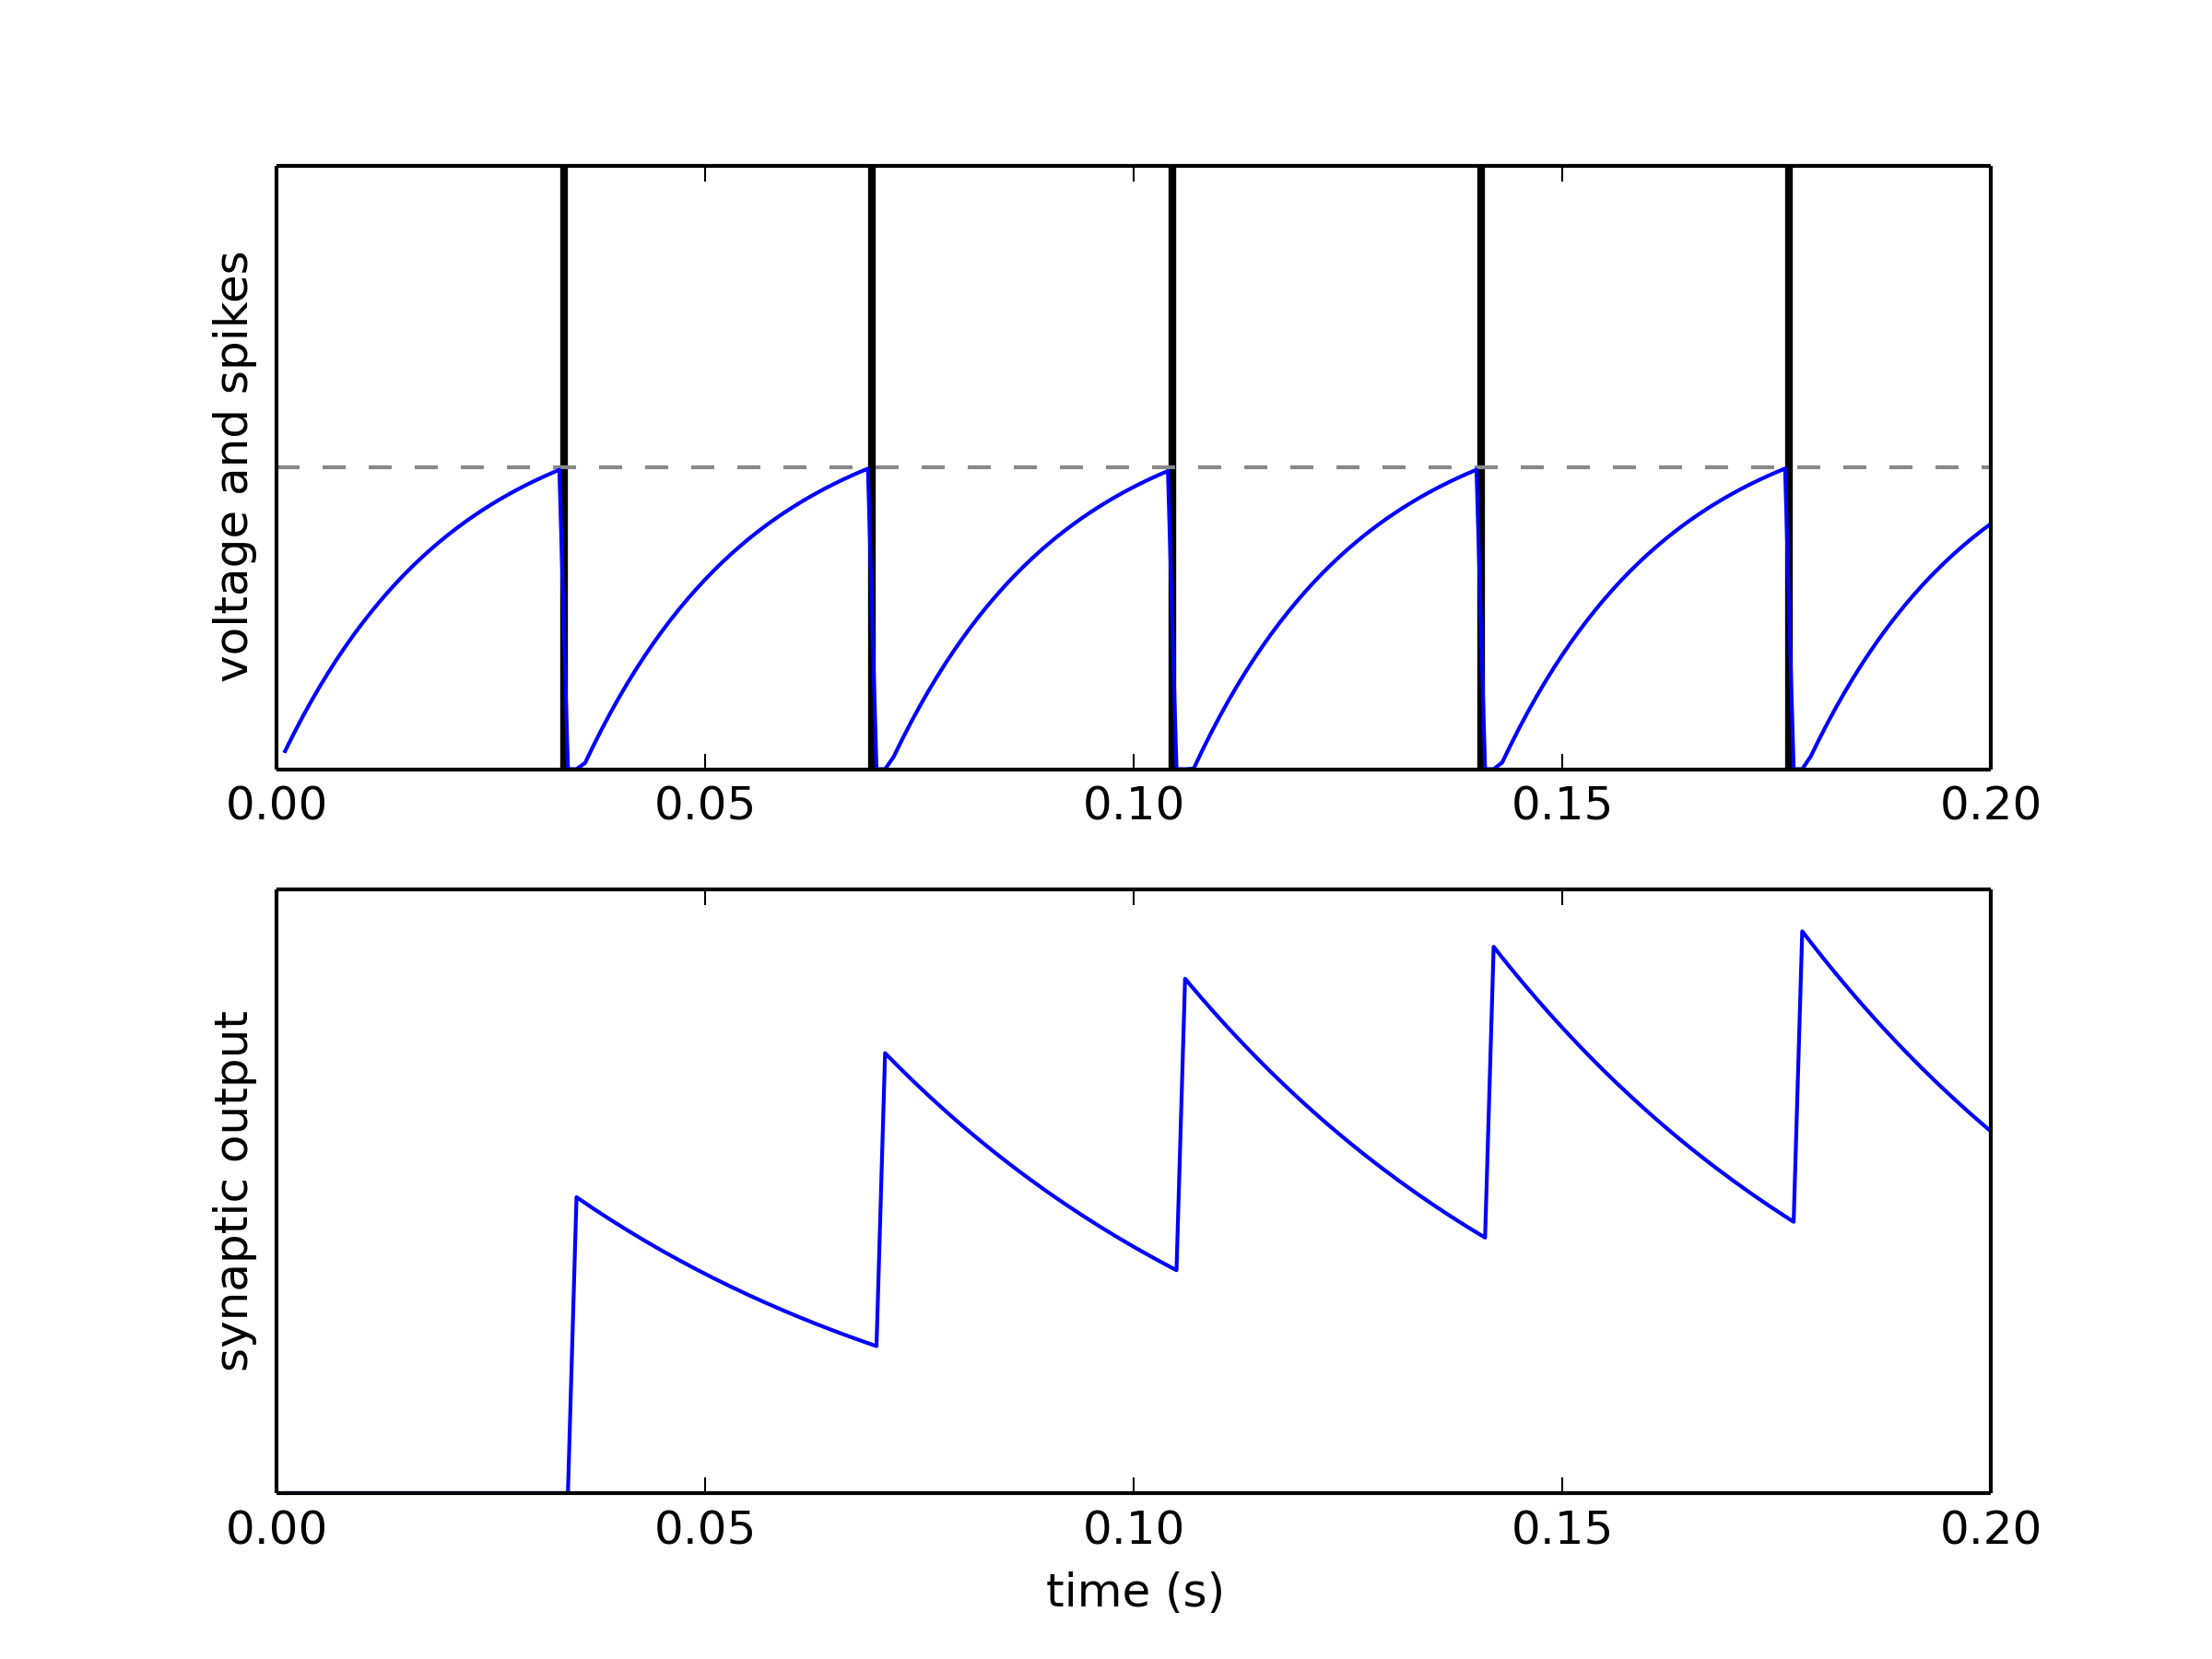
\includegraphics[width=3in]{neuron.png}
\caption{Voltage $V$, spiking activity and output of a single LIF neuron, given a constant input $I$.
SpiNNaker uses a simulation time step of $dt=0.001$.}
\label{Neuron}
\end{figure}

The goal of this work is to explore algorithms that can be usefully implemented
given hardware that efficiently implements neural networks of this form.  In
particular, we note that living creatures have both genetic, low-level 
hard-wired reflexes and they are also capable of developing novel associations 
between stimuli and responses that are entirely context-dependent. Behavioural 
studies indicate that they can learn to perform certain actions at certain 
times, through experience, overriding and building upon these low-level 
reflexes \cite{kim2007encoding}. 

However, for applied robotics applications, we do not want an approach where
learning is entirely autonomous and undirected (as in, for example, the neural
learning seen in Distributed Adaptive Control \cite{verschure2012distributed}). 
Instead, our approach is to inform neural learning by providing explicit
indications as to the instances where correct behaviour was achieved.  The 
approach described here is somewhat akin to reinforcement learning, but relies
only on positive examples, and can be explicitly shaped as desired.  This 
guides the learning and provides explicit control over the eventual behaviour. 

\section{Infrastructure}
\label{infrastructure}

[CHECK R3: "proposed approach is not well organised and written, therefore cannot see valuable novelty in manuscript."]

\subsection{eDVS}
The sensor system used here is the eDVS embedded dynamic vision 
sensor \cite{conradt2009embedded}, a silicon retina developed by iniLabs in 
collaboration with the Institute of Neuroinformatics at the University of 
Zurich and the ETH Zurich. This neuromorphic sensor is a 128x128-pixel camera. 
Instead of reporting frame-based data, it emits individual events when the 
relative brightness for any individual pixel increases or decreases. The eDVS 
provides high temporal resolution ($\sim$1us), low latency ($\sim$15us) and high dynamic 
range (120dB). The eDVS used here is an embedded version with an onboard 
microcontroller (NXP LPC4337), inertial measurement unit, multiple PWM control 
signals, and general-purpose I/O lines. The silicon retina is well-suited for 
integration with other neuromorphic hardware since it produces output in the 
form of spikes, which is the natural communication framework for spike-based 
neural processors. Furthermore, certain image processing algorithms can be 
implemented efficiently. For example, previous work \cite{muller2011miniature} 
has implemented high-speed tracking of flashing LEDs, and we use that algorithm 
here as sensory pre-processing.


\subsection{PushBot}
At the Technische Universit{\"a}t M{\"u}nchen, the Neuroscientific
System Theory group has developed a small tread-based robot built around the 
eDVS sensor, as shown in \figurename~\ref{fig_sim}. The robot provides two motors, a frequency-controllable laser pointer, two LEDs, and housing for power (4 AA batteries). The setup comes with a proprietary WLAN module, enabling streaming of sensor data and motor command to and from the robot over standard WiFi.

\begin{figure}[!t]
\centering
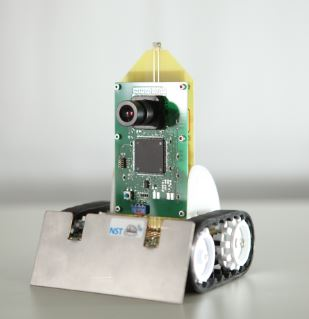
\includegraphics[width=2.5in]{Pushbot1CroppedCropped.jpg}
% where an .eps filename suffix will be assumed under latex, 
% and a .pdf suffix will be assumed for pdflatex; or what has been declared
% via \DeclareGraphicsExtensions.
\caption{The PushBot and the eDVS silicon retina.}
\label{fig_sim}
\end{figure}


\subsection{SpiNNaker}

The SpiNNaker multicore processor is developed by the University of Manchester 
and consists of 18 200MHz ARM968 cores on a single die \cite{furber2007neural, furber2014spinnaker}. 
The processors and inter-chip communication infrastructure are optimized for
massively parallel operations, with a target of a one-million-core machine.  Its
low power consumption means that a 48-chip SpiNNaker board with a total of 
864 processors uses under 40W of power. This system can be programmed directly 
in C or using the standard neural modeling API PyNN. However, for this work
we made use of the Nengo open-source neural compiler \cite{bekolay_nengo2014} 
(described below), and the custom Nengo backend that compiles high-level
neural models into optimized SpiNNaker code \cite{mundy2015}.

\subsection{Nengo and the Neural Engineering Framework}

The Neural Engineering Framework (NEF) is a general-purpose neural compiler 
that allows the user to define a high-level algorithm that is then compiled 
down to a neural approximation of that algorithm \cite{eliasmith2004neural}. 
This approach was originally meant for constructing complex biologically realistic neural 
models. Demonstrations of the use of Nengo for perception, cognition, and 
action encoding can be seen in Spaun, the first large-scale 
(2.5 million neuron) functional brain model capable of performing multiple 
tasks  \cite{eliasmith_largescale_2012}. 

The basic concept of modelling using the NEF is the same as most neural network
approaches: groups of neurons form distributed representations of their input,
and the weighted sum of the output from neurons is used to approximate
complex functions.  For example, in \figurename~\ref{Flow}, the six square
sensor boxes are the six values returned via the sensory preprocessing on the
PushBot robot, indicating the position ($x, y$) and certainty ($c$) information 
of two flashing lights (the laser pointer dot and the LED on the top of the
robot).  This information is encoded into the sensory neurons using random
connections; this ensures that there is a diverse and rich ``hidden layer''
representation in the sensory neurons, allowing a wide range of output
functions to be represented\footnote{It would, of course, be possible to use a
learning rule such as backpropagation of error to optimize these weights,
but we generally find this to be unnecessary}.

This means that different patterns of activity within
that group of neurons correspond to different vector values being represented.
This vector is (normally) of much smaller dimensionality than the number of 
neurons in the group, so the neural firing forms a redundant code for that 
vector. Each neuron in the group responds differently to the same input, due
to the random input connectivitty. Therefore, the redundant code can be thought of as a 
random projection from a low-dimensional space (the vector being represented) 
to a high-dimensional space (the neural activity). 

Connections out of a group of neurons implement functions on those represented 
vectors. That is, given some arbitrary function of the input vector, we can
find output connections from the neurons that will approximate that desired
function.  Importantly, due to 
the redundant code, these functions do not have to be linear functions; 
rather, any function can be specified, and the system will find the optimal
connections between neurons to approximate that function. The Neural Engineering 
Framework treats this as a least-squares minimization problem and finds the 
feed-forward linear synaptic connection weights between the individual neurons that will 
most closely approximate the desired nonlinear function. Furthermore, the NEF 
also indicates how recurrent connections can be found that will approximate 
any desired differential equation.  For both feed-forward and recurrent 
connections, the accuracy of the approximation will be dependent on the 
number of neurons and the function being approximated. 

As an example, consider a group of neurons storing three values: the $x,y$ 
position of an object and a certainty measure $c$ that the object is at that
location.  (This example comes from the output of the tracking algorithm 
for flashing LEDs \cite{muller2011miniature}).  In the NEF, we might use 100 
neurons to form a distributed representation of these three values 
(using more neurons would improve the accuracy of the representation).  Each
neuron would be given a random combination of inputs from the three dimensions,
resulting in a different pattern of firing for different vectors $(x,y,c)$.

Given this activity, we can then define connections to other groups of neurons
that compute functions of these values. For example, if we want a group of 
neurons $R$ to store the distance from the center of the visual field to the 
location of the LED, we could optimise the connections so
as to approximate: 
 
\begin{lstlisting}
    R = $\sqrt{x_{LED}^2 + y_{LED}^2}$
\end{lstlisting}

This would find synaptic connection weights between the group of neurons 
representing the LED data and the group of neurons representing the 
radius $R$ such that $R$ is driven to fire with whatever pattern represents 
the correct radius, given the current activity of the LED population. 

All of the neural systems described below are defined in this manner, using
the software package Nengo \cite{bekolay_nengo2014} developed specifically
for such neural network construction, along with its interface
for efficiently simulating such networks on SpiNNaker \cite{mundy2015}.

\section{Method}

The methodology used here is to start by building a neural system that
implements a base set of automatic ``reflex-like'' behaviors for the robot.
This is meant to correspond to the hardwired automatic responses found in
living creatures.  In addition to this, we will then add a learned system
where the robot must map its sensory state to the particular desired actions
for this condition.  This corresponds to learned associative responses
in animals.

[TODO R2: provide more insight into methodology, to reflect scientific paper rather than technical report]

\subsection{Initial Reflexive Control}
The first stage of this study requires a definition of the base set of simple 
behaviors and their triggering conditions, for a small mobile robot. These 
behaviors should be as simple as possible, since they must be hand-designed, 
but should provide a fairly rich repertoire of resulting actions. These can be 
thought of as, the basic, instinctive reflexes seen in living creatures. In
general, the first step in using this methodology is to define a collection
of these reflexes.

The first reflexive behavior is simply to go forward if there is no 
obstruction. To define this, we specify a function that uses sensor data to 
compute the current strength $S$ of an action (i.e. $0$ to $1$). In this 
case, the visual position of the dot caused by the laser pointer mounted on
the robot can be used as a simple range 
detector: if it is lower than some threshold, the robot is near a wall and 
should not go forward. If it is higher than that threshold, it is safe to 
go forward: 

\begin{lstlisting}
	S[0] = 1 if $y_{LASER} > -0.6$ else 0
\end{lstlisting}

To complete this basic behavior, we define the motor output $M$ as a 
function of $S$. In this case, we want to drive both wheel motors forward 
when the action has a high strength.

\begin{lstlisting}
	M = [1, 1] $\cdot$ S[0]
\end{lstlisting}

The next basic reflexive action is to back up when we are too close to an 
obstacle. This is again detected by using the visual location of the dot
shown by the laser pointer.  If this is very low in the visual field, or if
it is not visible at all (i.e. the dot is below the field of view of the camera)
then the robot should back up.  This gives the following rule:

\begin{lstlisting}
	S[1] = 1 if $y_{LASER} < -0.8$ or $c_{LASER} < 0$ else 0
	M = [-1, -1] $\cdot$ S[1]
\end{lstlisting}

The final basic actions are: turn left or right when close to an obstacle. 

\begin{lstlisting}
	S[2] = 1 if $y_{LASER} < -0.8$ else 0
	M = [-1, 1] $\cdot$ S[2]

	S[3] = 1 if $y_{LASER} < -0.8$ else 0
	M = [1, -1] $\cdot$ S[3]
\end{lstlisting}

However, these last two actions should not both be performed at the same time,
since this would cause the robot to stay in place, rather than turning one
direction or the other. To specify this, we can define connections that relate 
the strengths of different actions to each other.

\begin{lstlisting}
	S[2] = -S[3]
	S[3] = -S[2]
\end{lstlisting}

This means that whenever $S[2]$ is positive, it will force $S[3]$ towards $0$, 
and similarly $S[3]$ will drive $S[2]$ towards $0$.  This implements a classic
neural competition, meaning that only one of the two actions will have a large
value at a particular time.

Now that these reflex actions have been defined in these simple terms, we use
Nengo to build neural networks that approximate each of these rules.  Groups
of neurons are defined to store the sensory state, the motor output, and the 
strengths of each action. The connections between the groups of neurons are 
set to approximate each of the above functions, resulting in the neural 
system shown in \figurename~\ref{Flow}. 

To understand the resulting basic reflexive behavior,
two important aspects of NEF must be considered. First, due to the neural 
representation scheme, when there are multiple inputs to a neural population, 
the value represented will be the sum of the input values. In other words. the 
motor output will be the sum of all the connections: $S[0]$, $S[1]$, $S[2]$, and $S[3]$ to $M$. 
Second, the NEF approximations of the desired functions will be \textit{smooth}. 
That is, instead of implementing the exact functions specified above, the 
actual behavior will be much more gradual. 

\begin{figure}[!t]
\centering
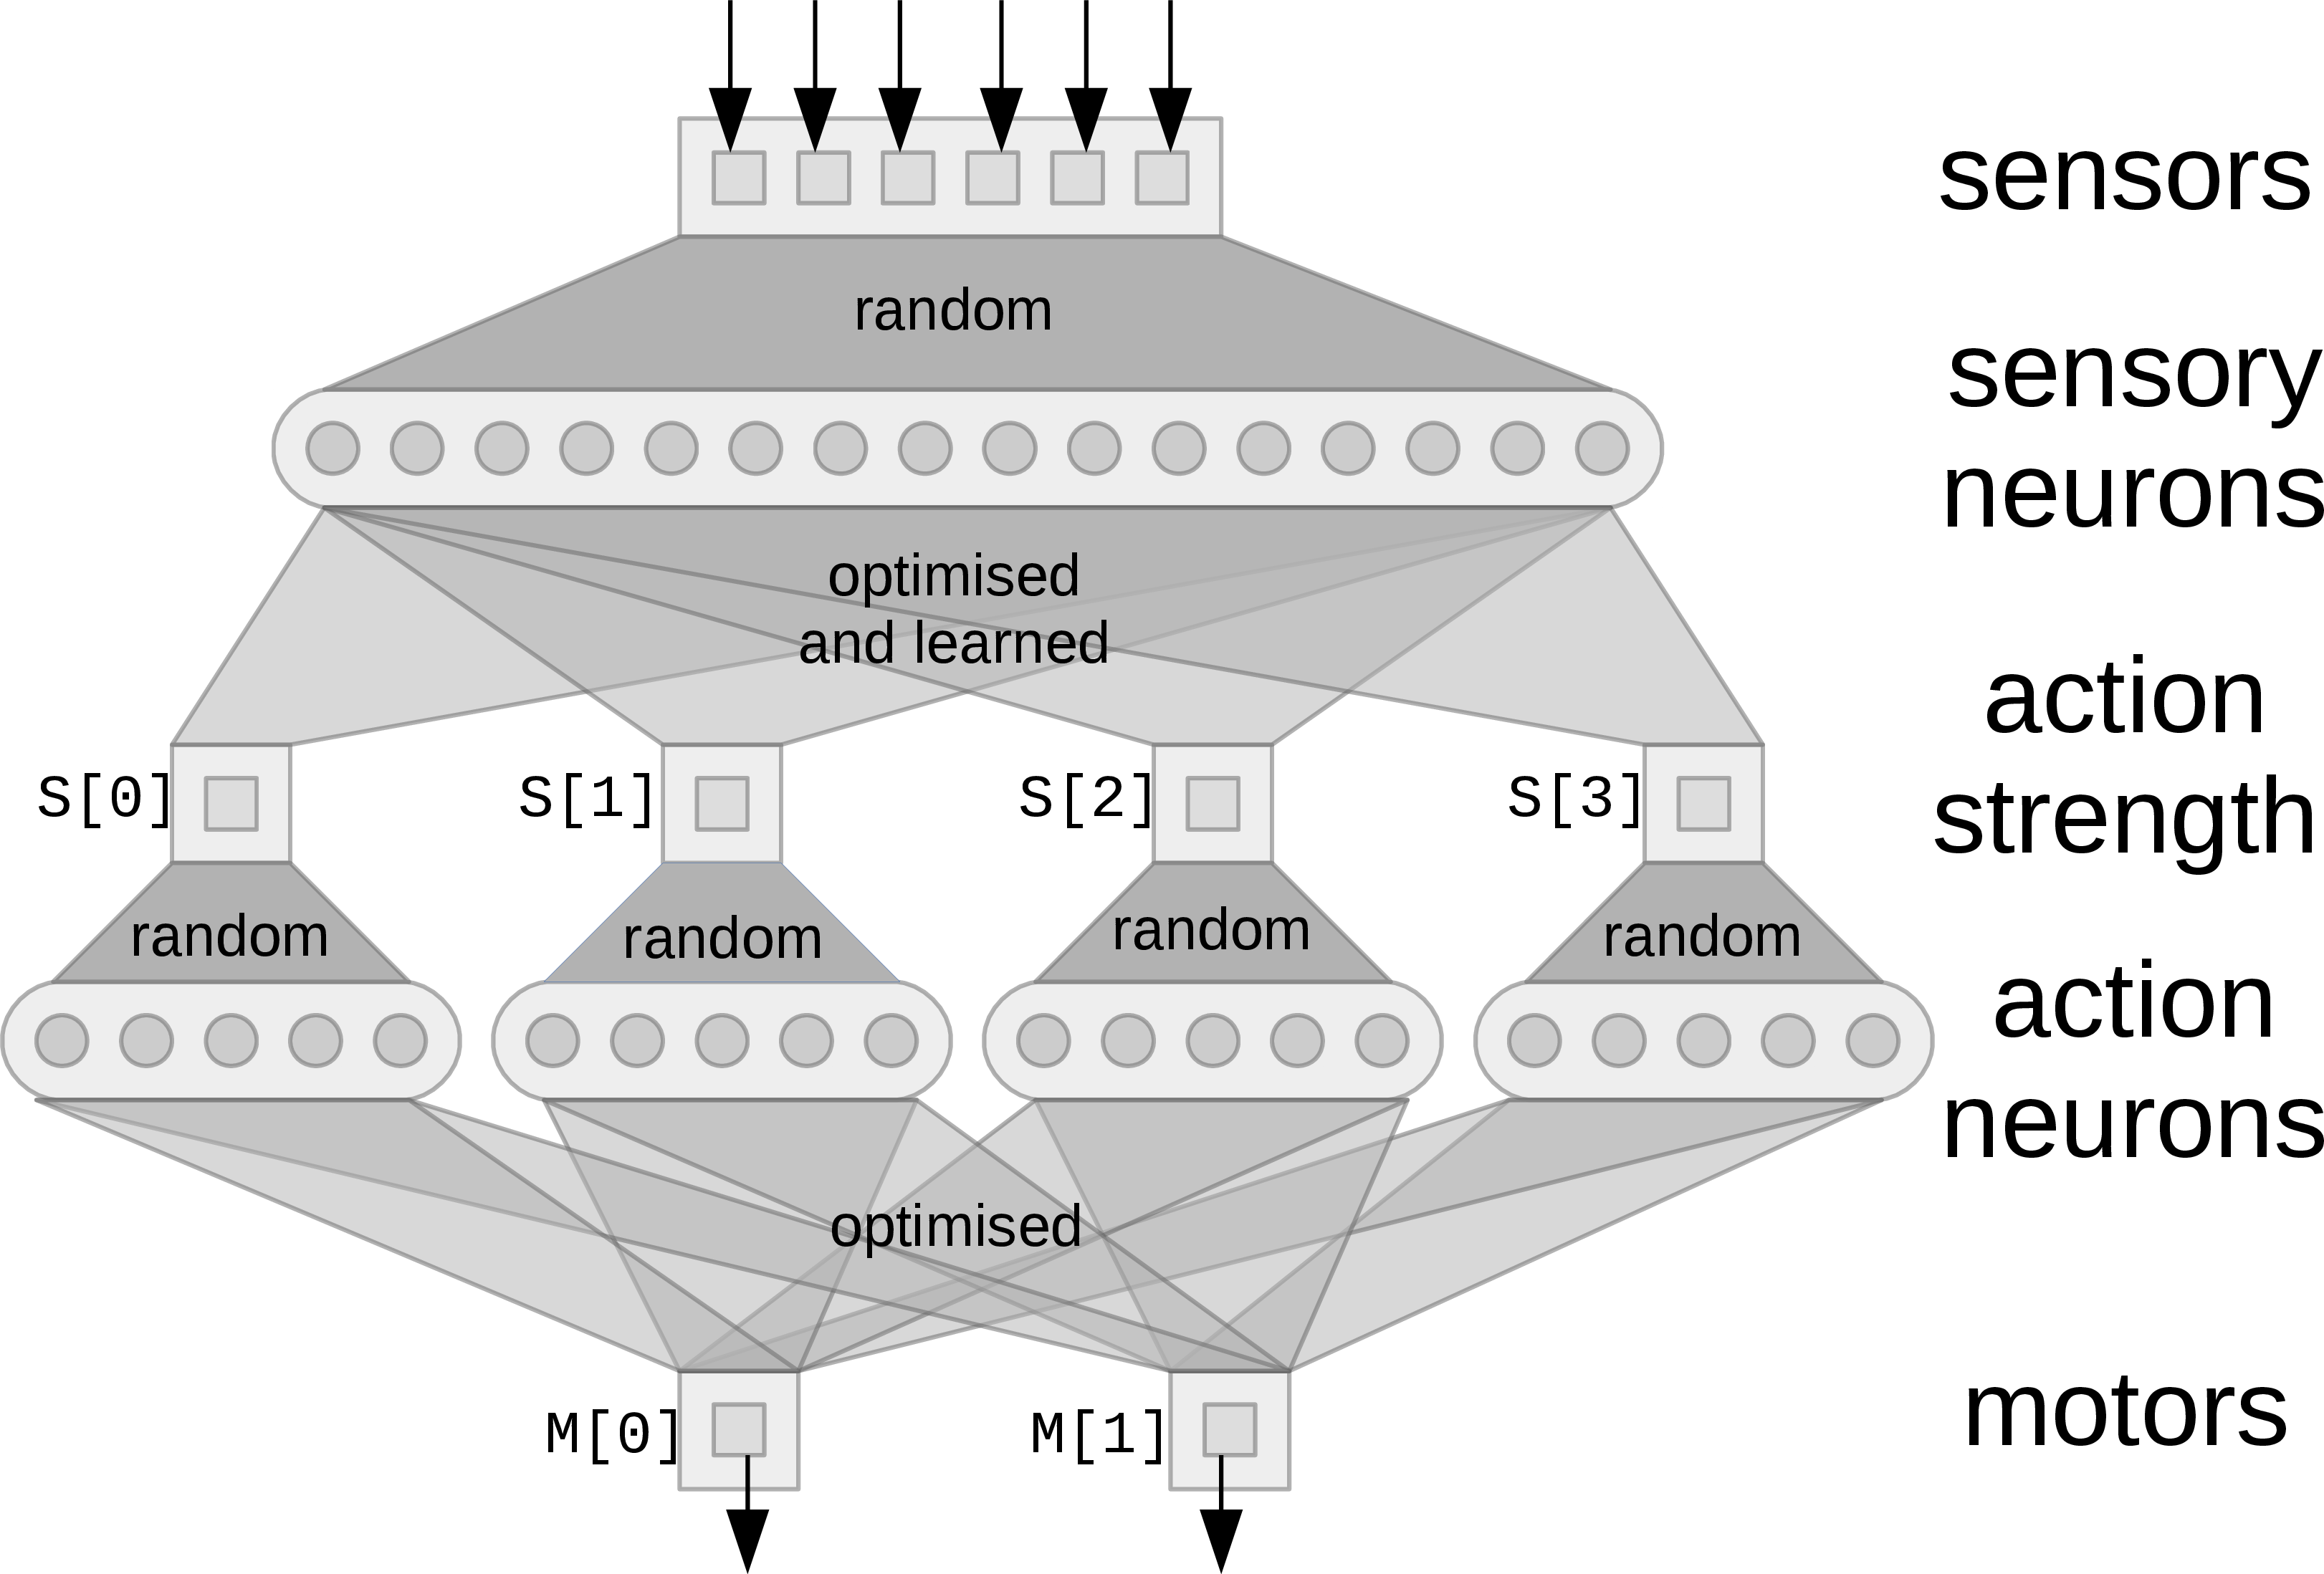
\includegraphics[width=3in]{network.png}
\caption{A network implementing basic reactive control. Square boxes are the
values being represented by the neurons (circles).  Random connectivity
ensures the neurons form a distributed representation of the vector values
that are their input.  The optimised output connections are solved for
using least-squares minimization to approximate the functions listed in
the text.  Learned connections are added afterwards, as discussed in 
section \ref{learning}.}
\label{Flow}
\end{figure}


\begin{figure}[!t]
\centering
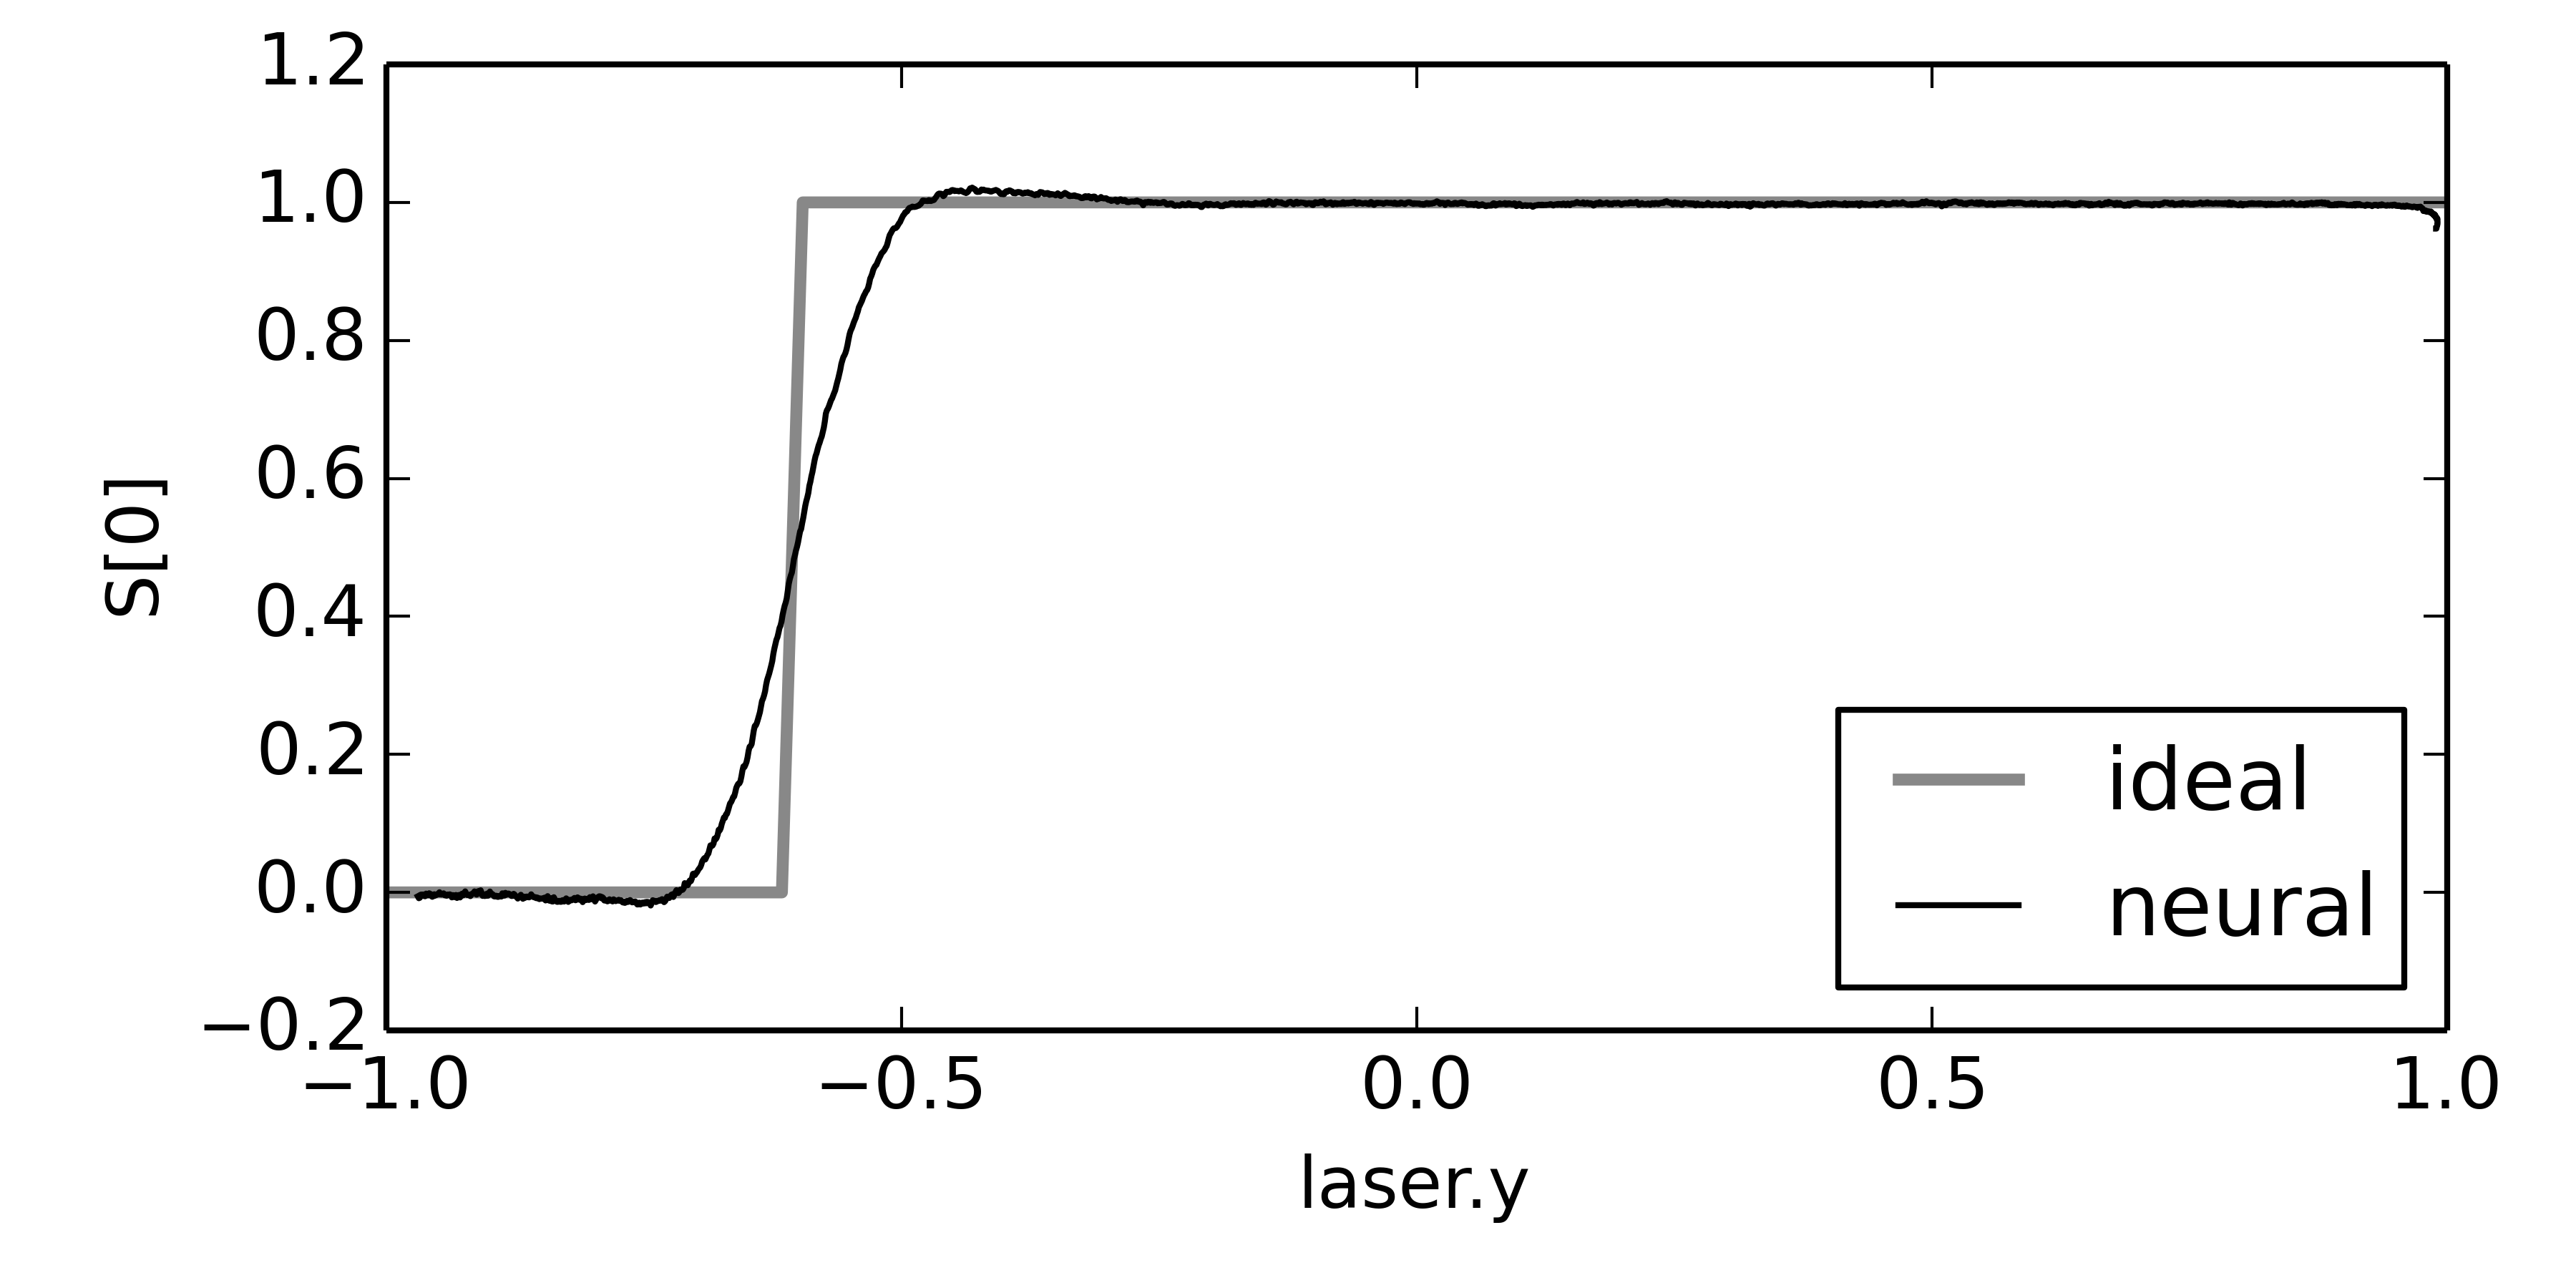
\includegraphics[width=2.5in]{smoothing.png}
% where an .eps filename suffix will be assumed under latex, 
% and a .pdf suffix will be assumed for pdflatex; or what has been declared
% via \DeclareGraphicsExtensions.
\caption{Neural approximation with the NEF. When connections between neural groups are optimized to approximate a function, the result is a smooth version of that function. As the number of neurons is increased, this neural approximation will approach the ideal function.}
\label{NEF}
\end{figure}

For example, the input function to 
the $S[0]$ population is supposed to compute ``$1$ if $y_{LASER} > -0.6$ else $0$''. 
Instead of implementing this exact function, the neurons will instead implement
a smoothed approximation of this step function, as shown in
\figurename~\ref{NEF}.

The result is a small spiking neural network control system that performs very 
simple obstacle avoidance. Due to the smoothing inherent in the NEF neural 
approximation of the above functions, the robot gradually transitions between 
behaviors. This means that it will automatically slow when approaching a wall, 
even though we have not explicitly built reflexes to do so.  

\begin{figure}[!t]
\centering
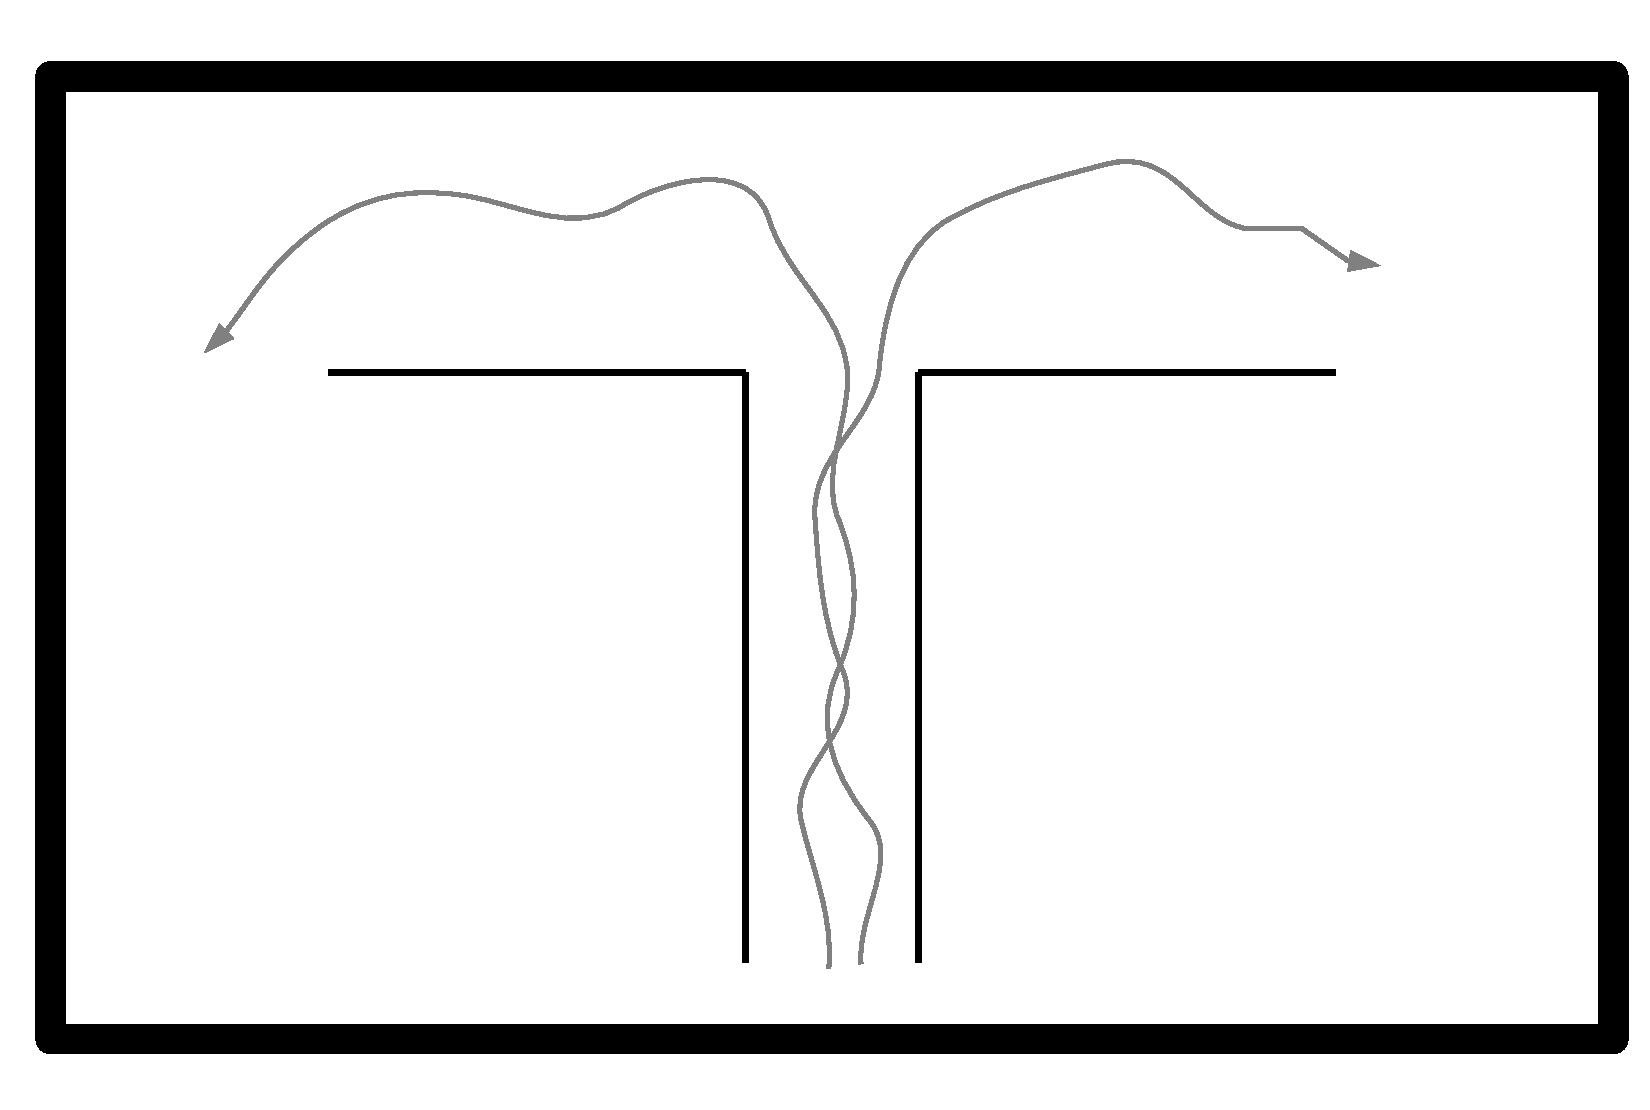
\includegraphics[width=2.5in]{tmazeRev.pdf}
% where an .eps filename suffix will be assumed under latex, 
% and a .pdf suffix will be assumed for pdflatex; or what has been declared
% via \DeclareGraphicsExtensions.
\caption{The T-Maze environment. The robot starts at the bottom of the T shape.}
\label{Tmaze}
\end{figure}

When it reaches a wall, it will then turn in a random direction. This randomness will be due 
entirely to sensory noise, as there is no stochasticity in the neural model 
itself. Once it has chosen a particular direction to turn, i.e. once 
either $S[2]$ or $S[3]$ has a high value, it will continue to turn in that 
direction until there is no longer an obstacle in front of it. All actions 
transpire without human interference. The only hardcoded input are the initial 
thresholds that provide information as to whether an action is, in fact, 
correct given the current sensory state. These actions demonstrate obstacle 
avoidance and simple decision making, in much the same way as animal behavior 
studies \cite{kim2007encoding}. 

The core idea is that this set of behaviors is a bare minimum, sufficient to
allow the robot to move throughout its environment without human intervention.
As with animal behaviour, this allows the robot to have a basic set of automatic
decision-making rules that apply in novel situations where there is not yet
any learned response.  Using these reflexive rules, the robot makes ``accidental''
decisions (turning left in some situations and turning right in others, for
example), which we will then use to further train the robot's behavior, as
discussed in the next section.


\subsection{Initial behavior}

To examine the model's behavior, we used a standard T-maze
environment (\figurename~\ref{Tmaze}). When placed at the bottom
of the T-maze, the robot navigates forward, avoids the
walls, reaches the choice point, and turns left or right.
Typical trajectories are shown in \figurename~\ref{React}, which indicates
the motor outputs over time. Since the robot uses tank-style treads, the 
two motor output values are the left and right motor speeds, respectively. 
For clarity, here we plot the overall speed as the sum of M[0] (left motor) 
and M[1] (right motor), while the rotation rate is the difference between the two. 
Motor output values of typical individual runs are plotted along with an overall 
mean value (with 95\% bootstrap confidence interval). All values are Gaussian 
filtered with $\sigma=0.15s$ for visual clarity.


\begin{figure}[!t]
\centering
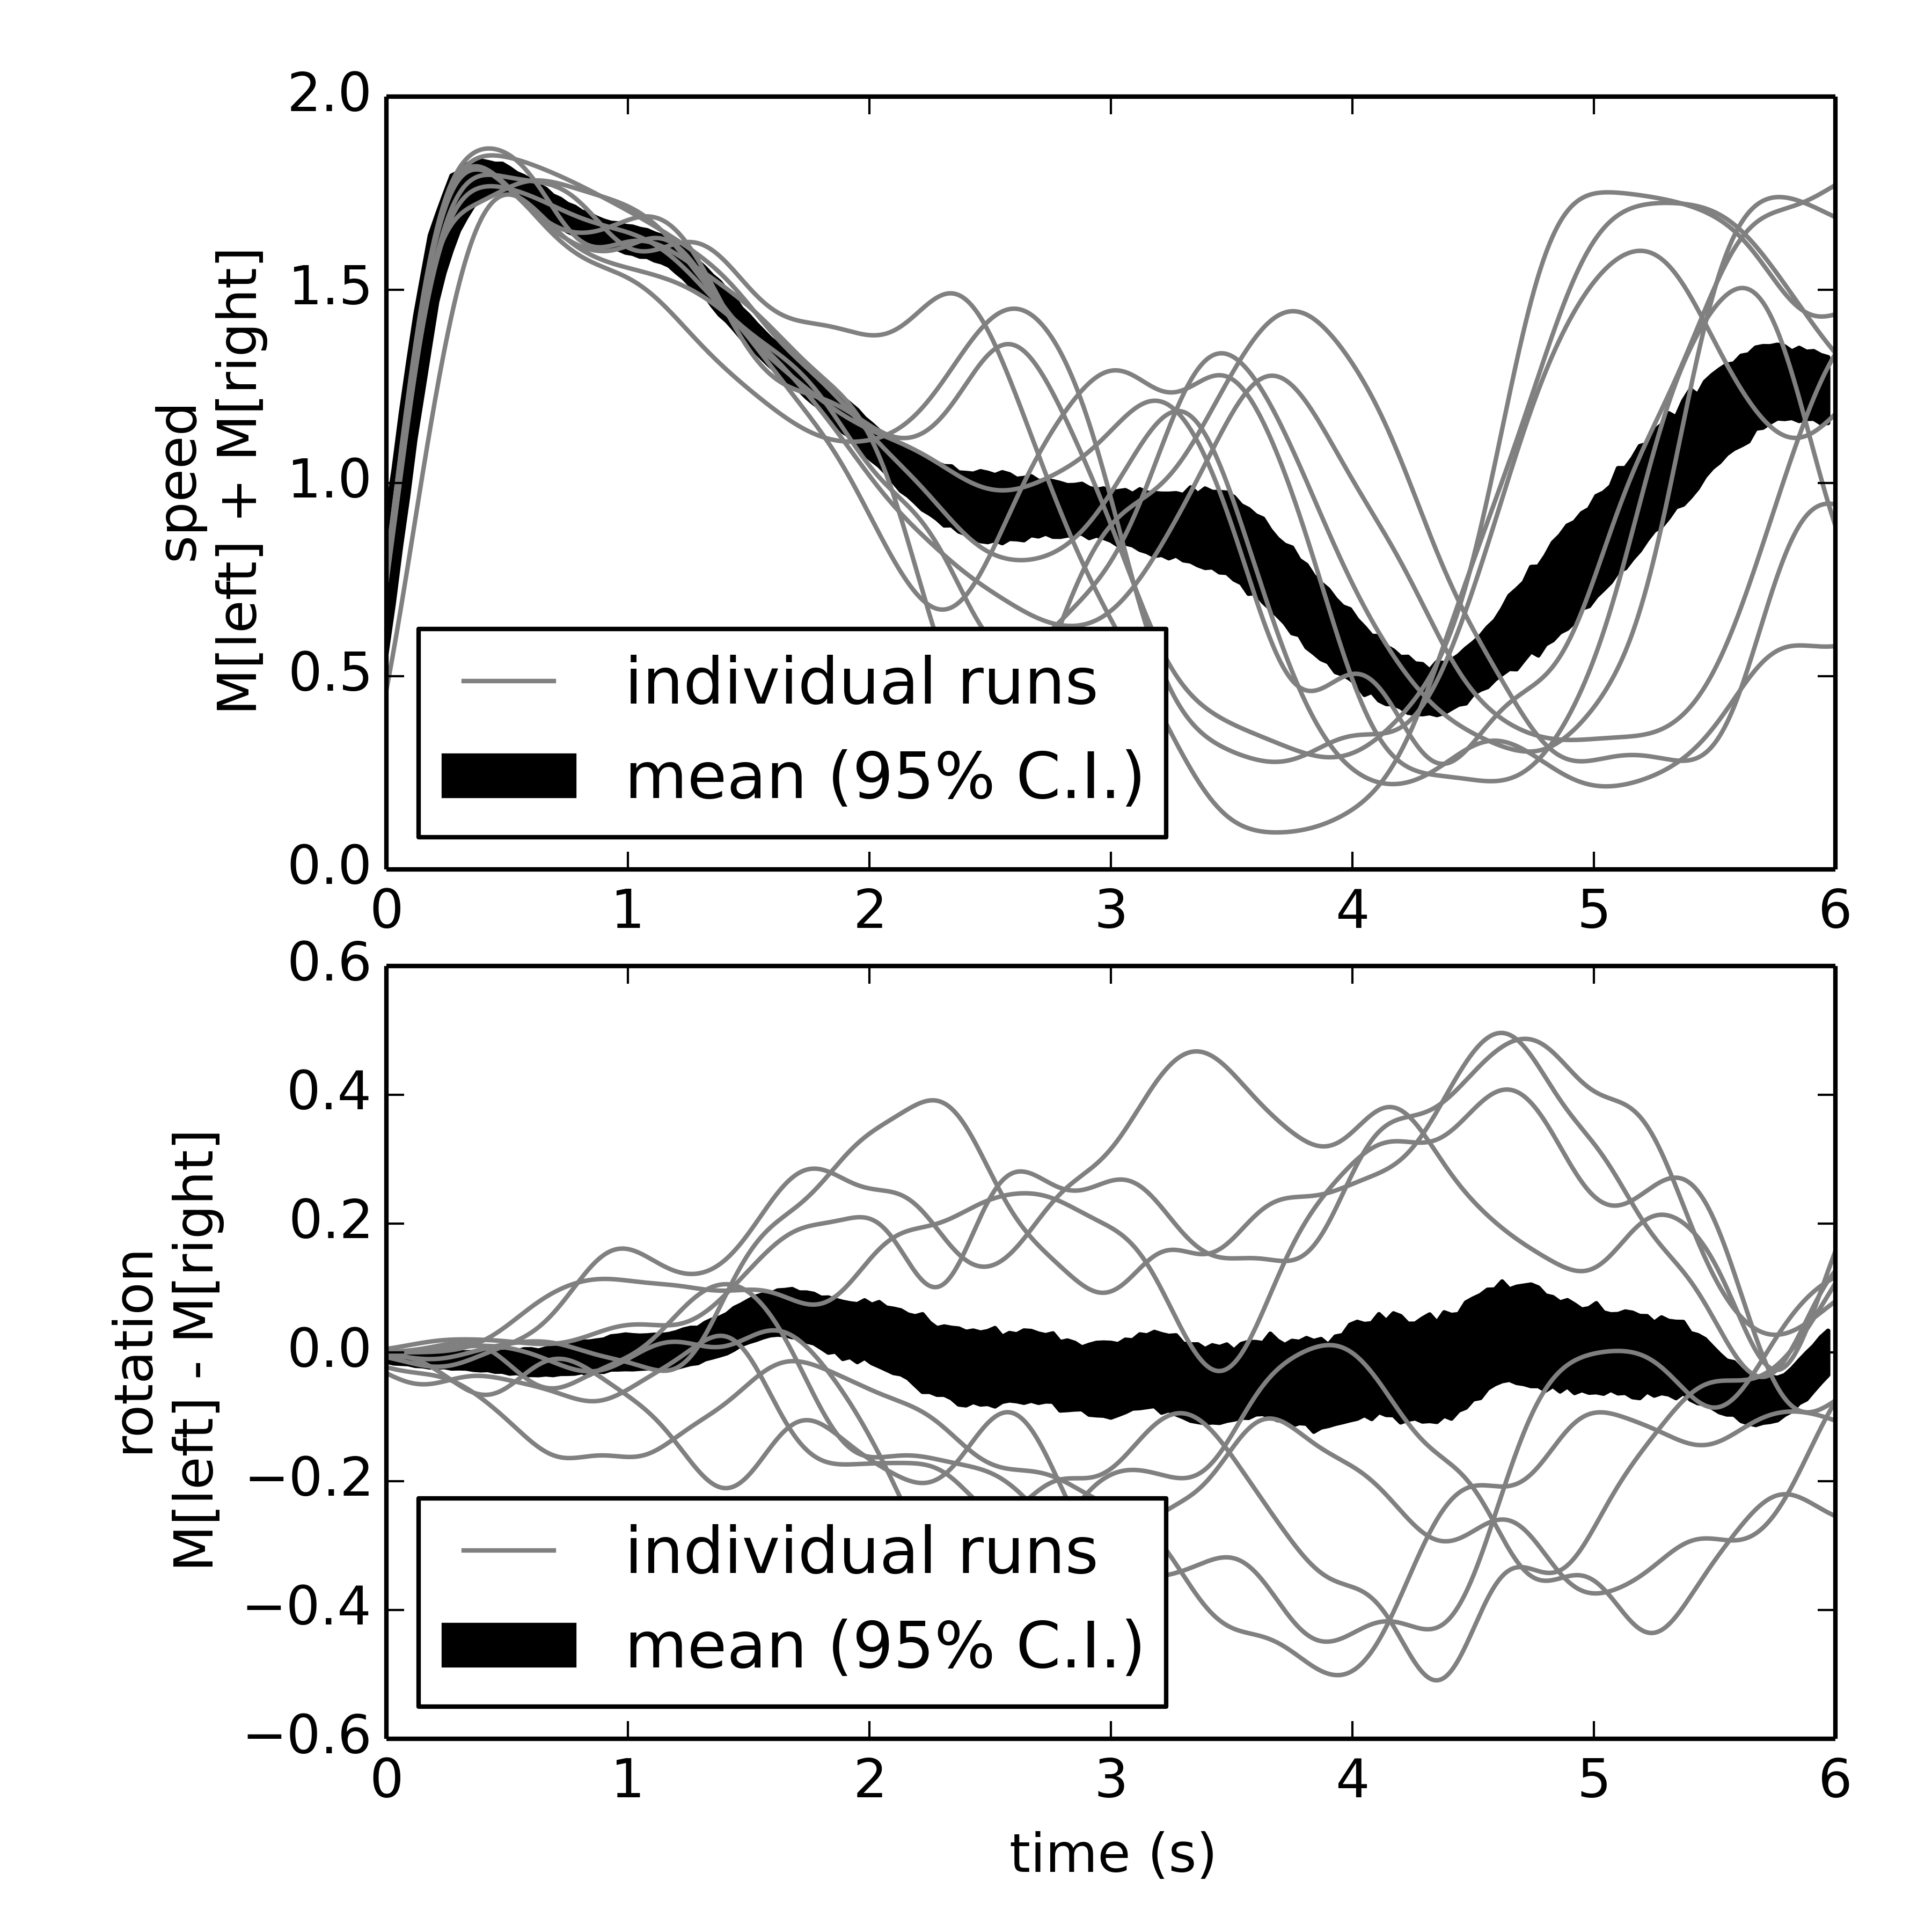
\includegraphics[width=2.5in]{basic/basic.png}
\caption{Behavior of reactive control model over multiple runs. The speed (top graph) is high at the beginning, then slows as it turns either left or right (bottom graph). While on any individual run the robot tends to turn consistently either left or right, the overall average is zero turning (black area in bottom graph; area is 95\% bootstrap confidence interval).}
\label{React}
\end{figure}




\subsection{Serendipitous Offline Learning} \label{learning}

While the above approach is sufficient for implementing simple behaviors, it requires the developer to define explicit rules mapping sensory states to actions. In this section, we build upon these
rules in a less explicit manner, allowing us to create more complex behavior
without hard-coding any additional rules.  In complex situations, it may not be 
feasible for action rules, such as the ones defined above, to be hard coded. Instead,
we can also define \textit{implicit} action rules. The basic idea is to allow
the robot to explore its environment, but whenever it happens to accidentally
do whatever action we want it to do, we record the sensory and motor 
values and \textit{use those values to define a new rule}.

For example, consider the simple case where we want the robot to always turn left at 
the intersection, rather than randomly turning either left or right. Recording 
the sensory data and the strength of each action $S$ while the robot is 
performing its initial basic behavior, we find instances where the robot 
performs the desired action (turning left). We call these the \textit{positive 
examples}. In this case, we consider the four individual runs shown in \figurename~\ref{React} where the robot's rotation tended to remain positive.  The data from runs where it turned right are removed.  The data from these positive examples can 
be thought of as long sequences of state-action pairs, indicating what action 
to perform in what state. Given this, we add new connections from sensors to 
the action strength populations. Instead of explicitly indicating what functions 
to approximate on these connections, we instead use the data gathered from
the robot itself to be the target function that the neurons must approximate.

At first glance, it seems as if these new connections would just end up being 
exactly the same as the original reflexive control connections. However, the 
key difference here is that these new connections will also take into 
account \textit{other sensory states}, not considered in the original 
hand-designed reflexive rules. In other words, these new connections will 
cause the robot to be more likely to perform the actions we desire whenever it is in a sensory state similar to those seen in the positive examples. 
Importantly, this will happen without any explicit indication of exactly what 
sensory states should trigger what actions.  This allows the system to
discover more complex rules than could be reasonably manually hand-designed.

\section{Results}

The result of this training is shown in \figurename~\ref{Left}. Unlike 
\figurename~\ref{React} this shows the robot consistently turning to the left about 
two seconds into the task (the average time for the robot to reach the end of the corridor).

\begin{figure}[!t]
\centering
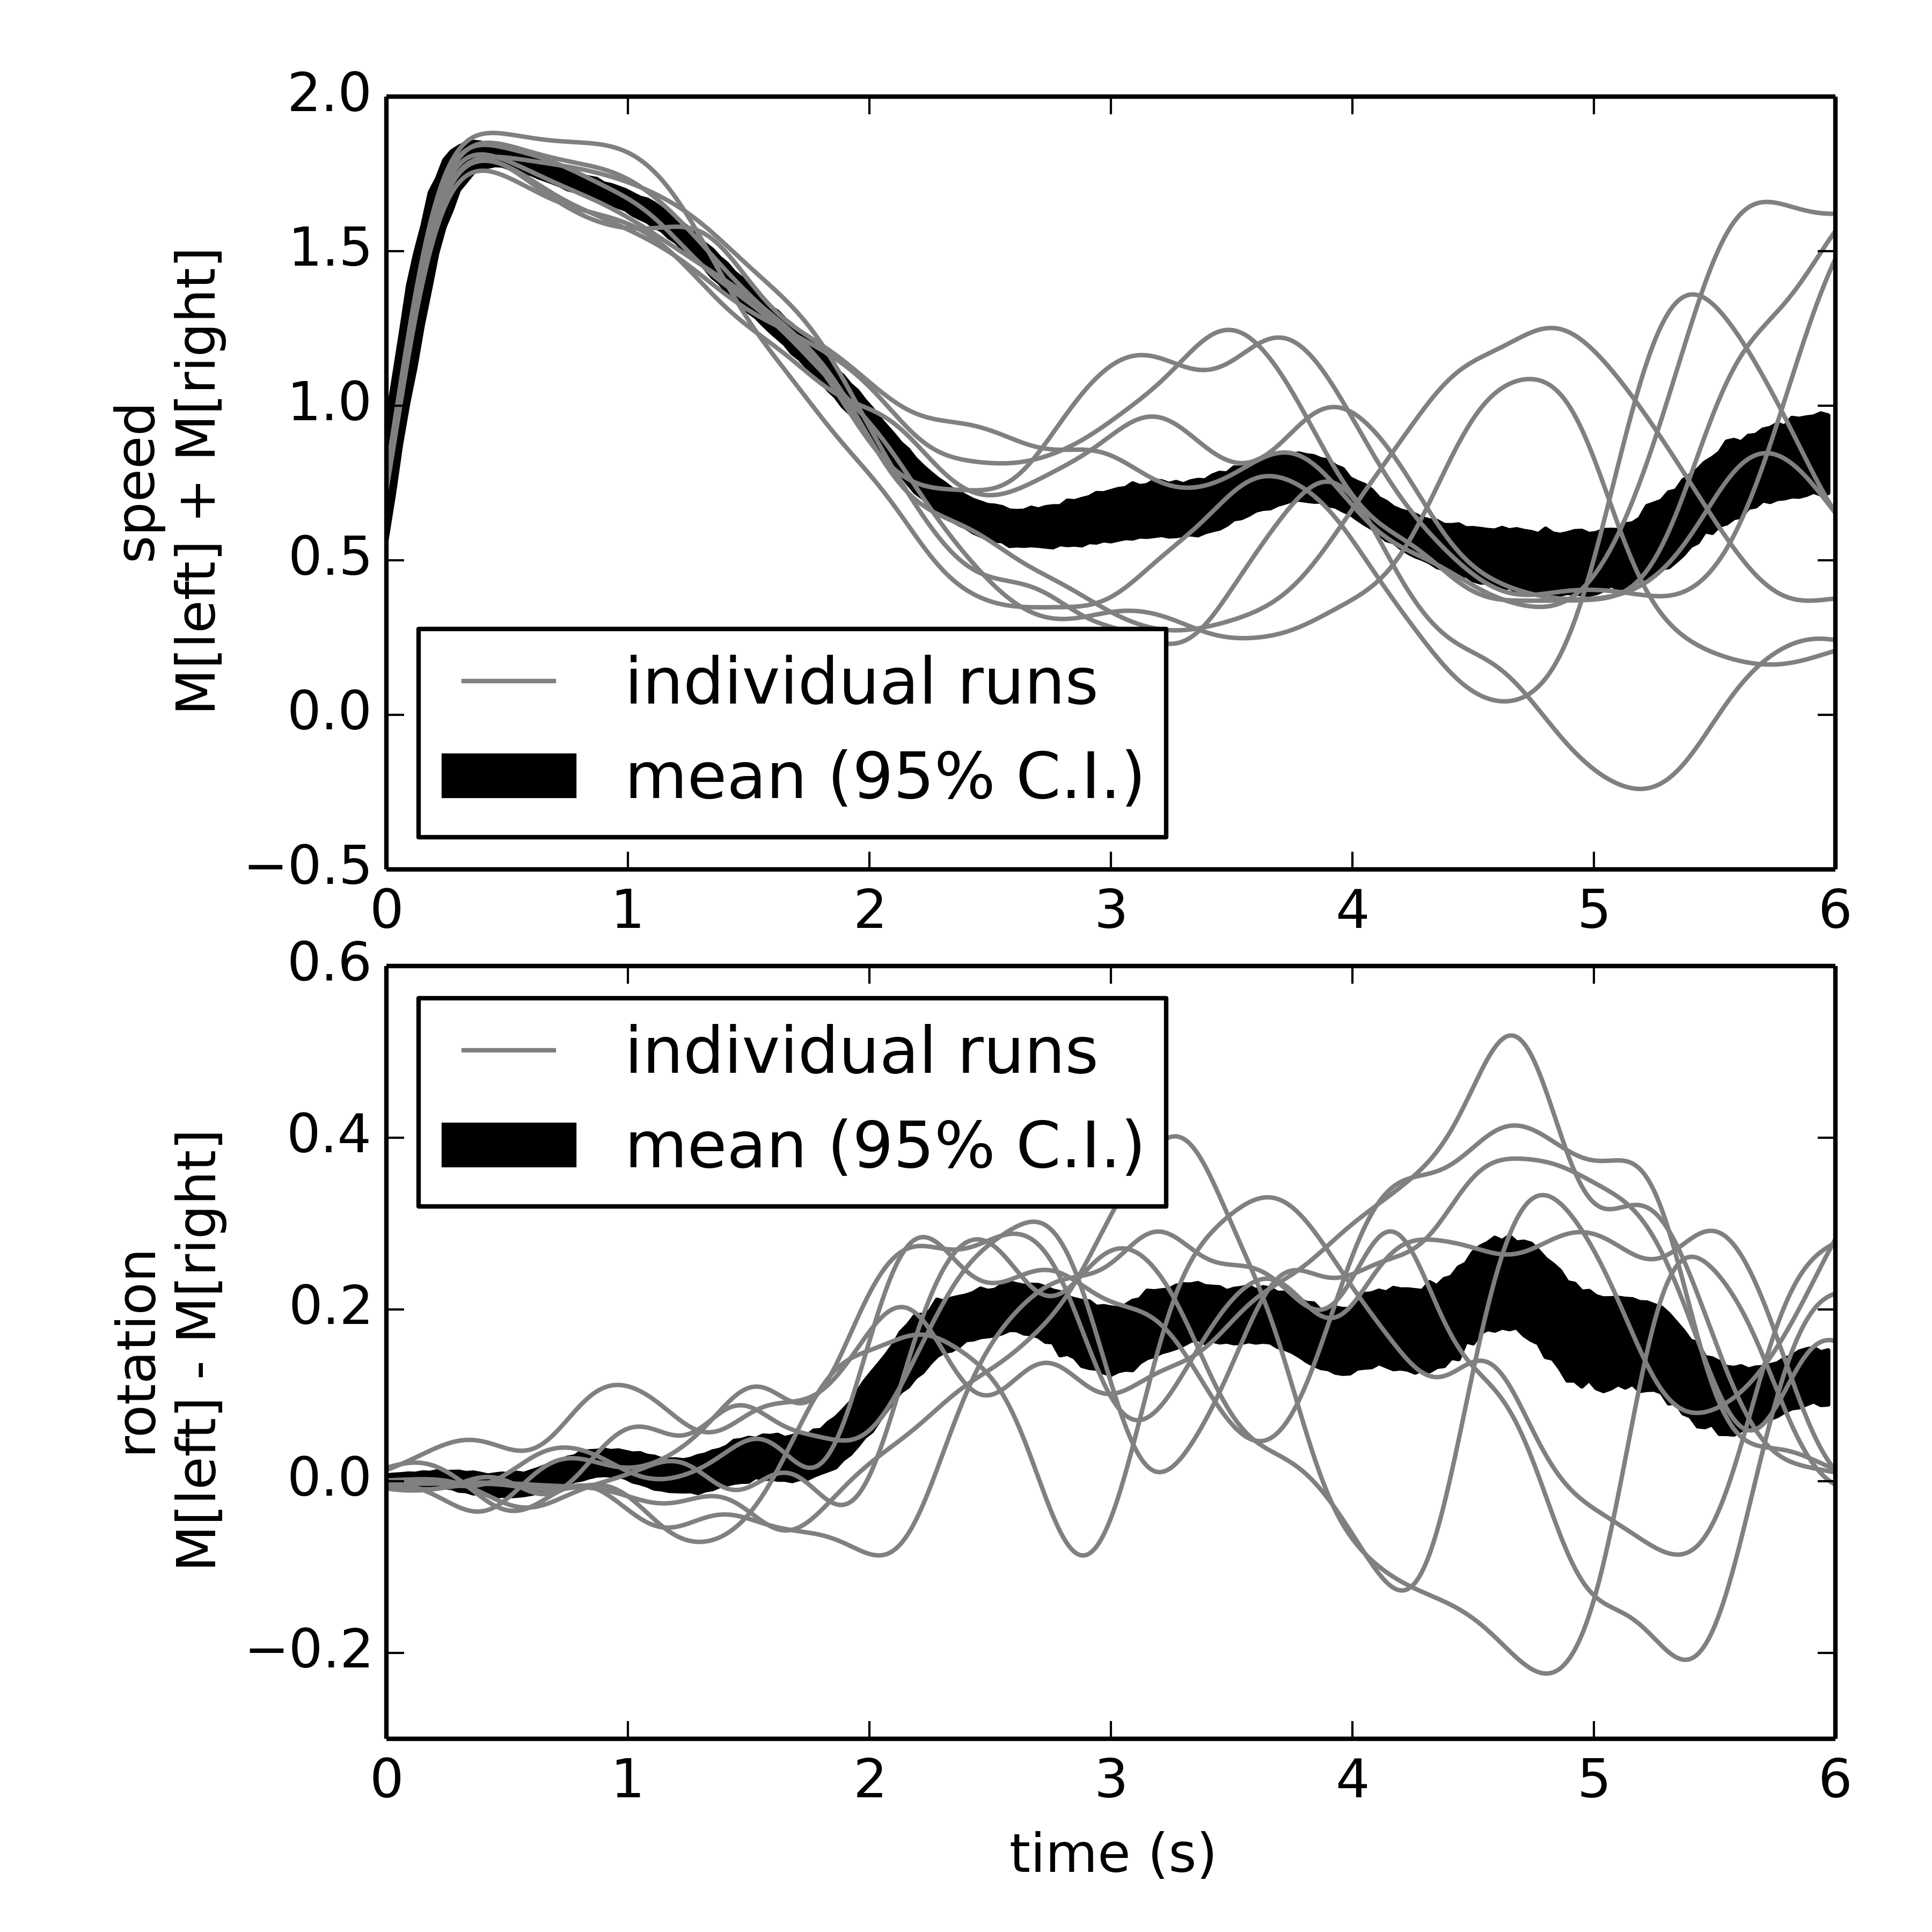
\includegraphics[width=2.5in]{learn-left/learnleft.png}
% where an .eps filename suffix will be assumed under latex, 
% and a .pdf suffix will be assumed for pdflatex; or what has been declared
% via \DeclareGraphicsExtensions.
\caption{Behavior after learning to turn left. By adding connections optimized to approximate situations where the robot behaved appropriately, we implicitly program the robot to map its sensory states to its actions as desired.}
\label{Left}
\end{figure}

\subsection{Learning Sensory Conditions}

The initial example of learning to turn left is not particularly complex. 
However, we can use exactly the same process to produce more complex behavior.
To demonstrate this, we now sometimes place a \textit{mirror} at the intersection.
Initially, the robot will ignore the mirror and just use its standard random
reflexive navigation.  We now choose as our positive examples situations where
the robot turned right when there was a mirror, and situations where it turned
left when there was no mirror.

Adding a learned connection that attempts to approximate those positive
examples means that the neural connections now need to change their outputs
depending on whether the mirror is present or not.  \figurename~\ref{Right} shows 
that the robot can successfully learn to recognize and respond to mirrors,
given only this simple learning rule on top of its basic reflexive rules.

\begin{figure}[!t]
\centering
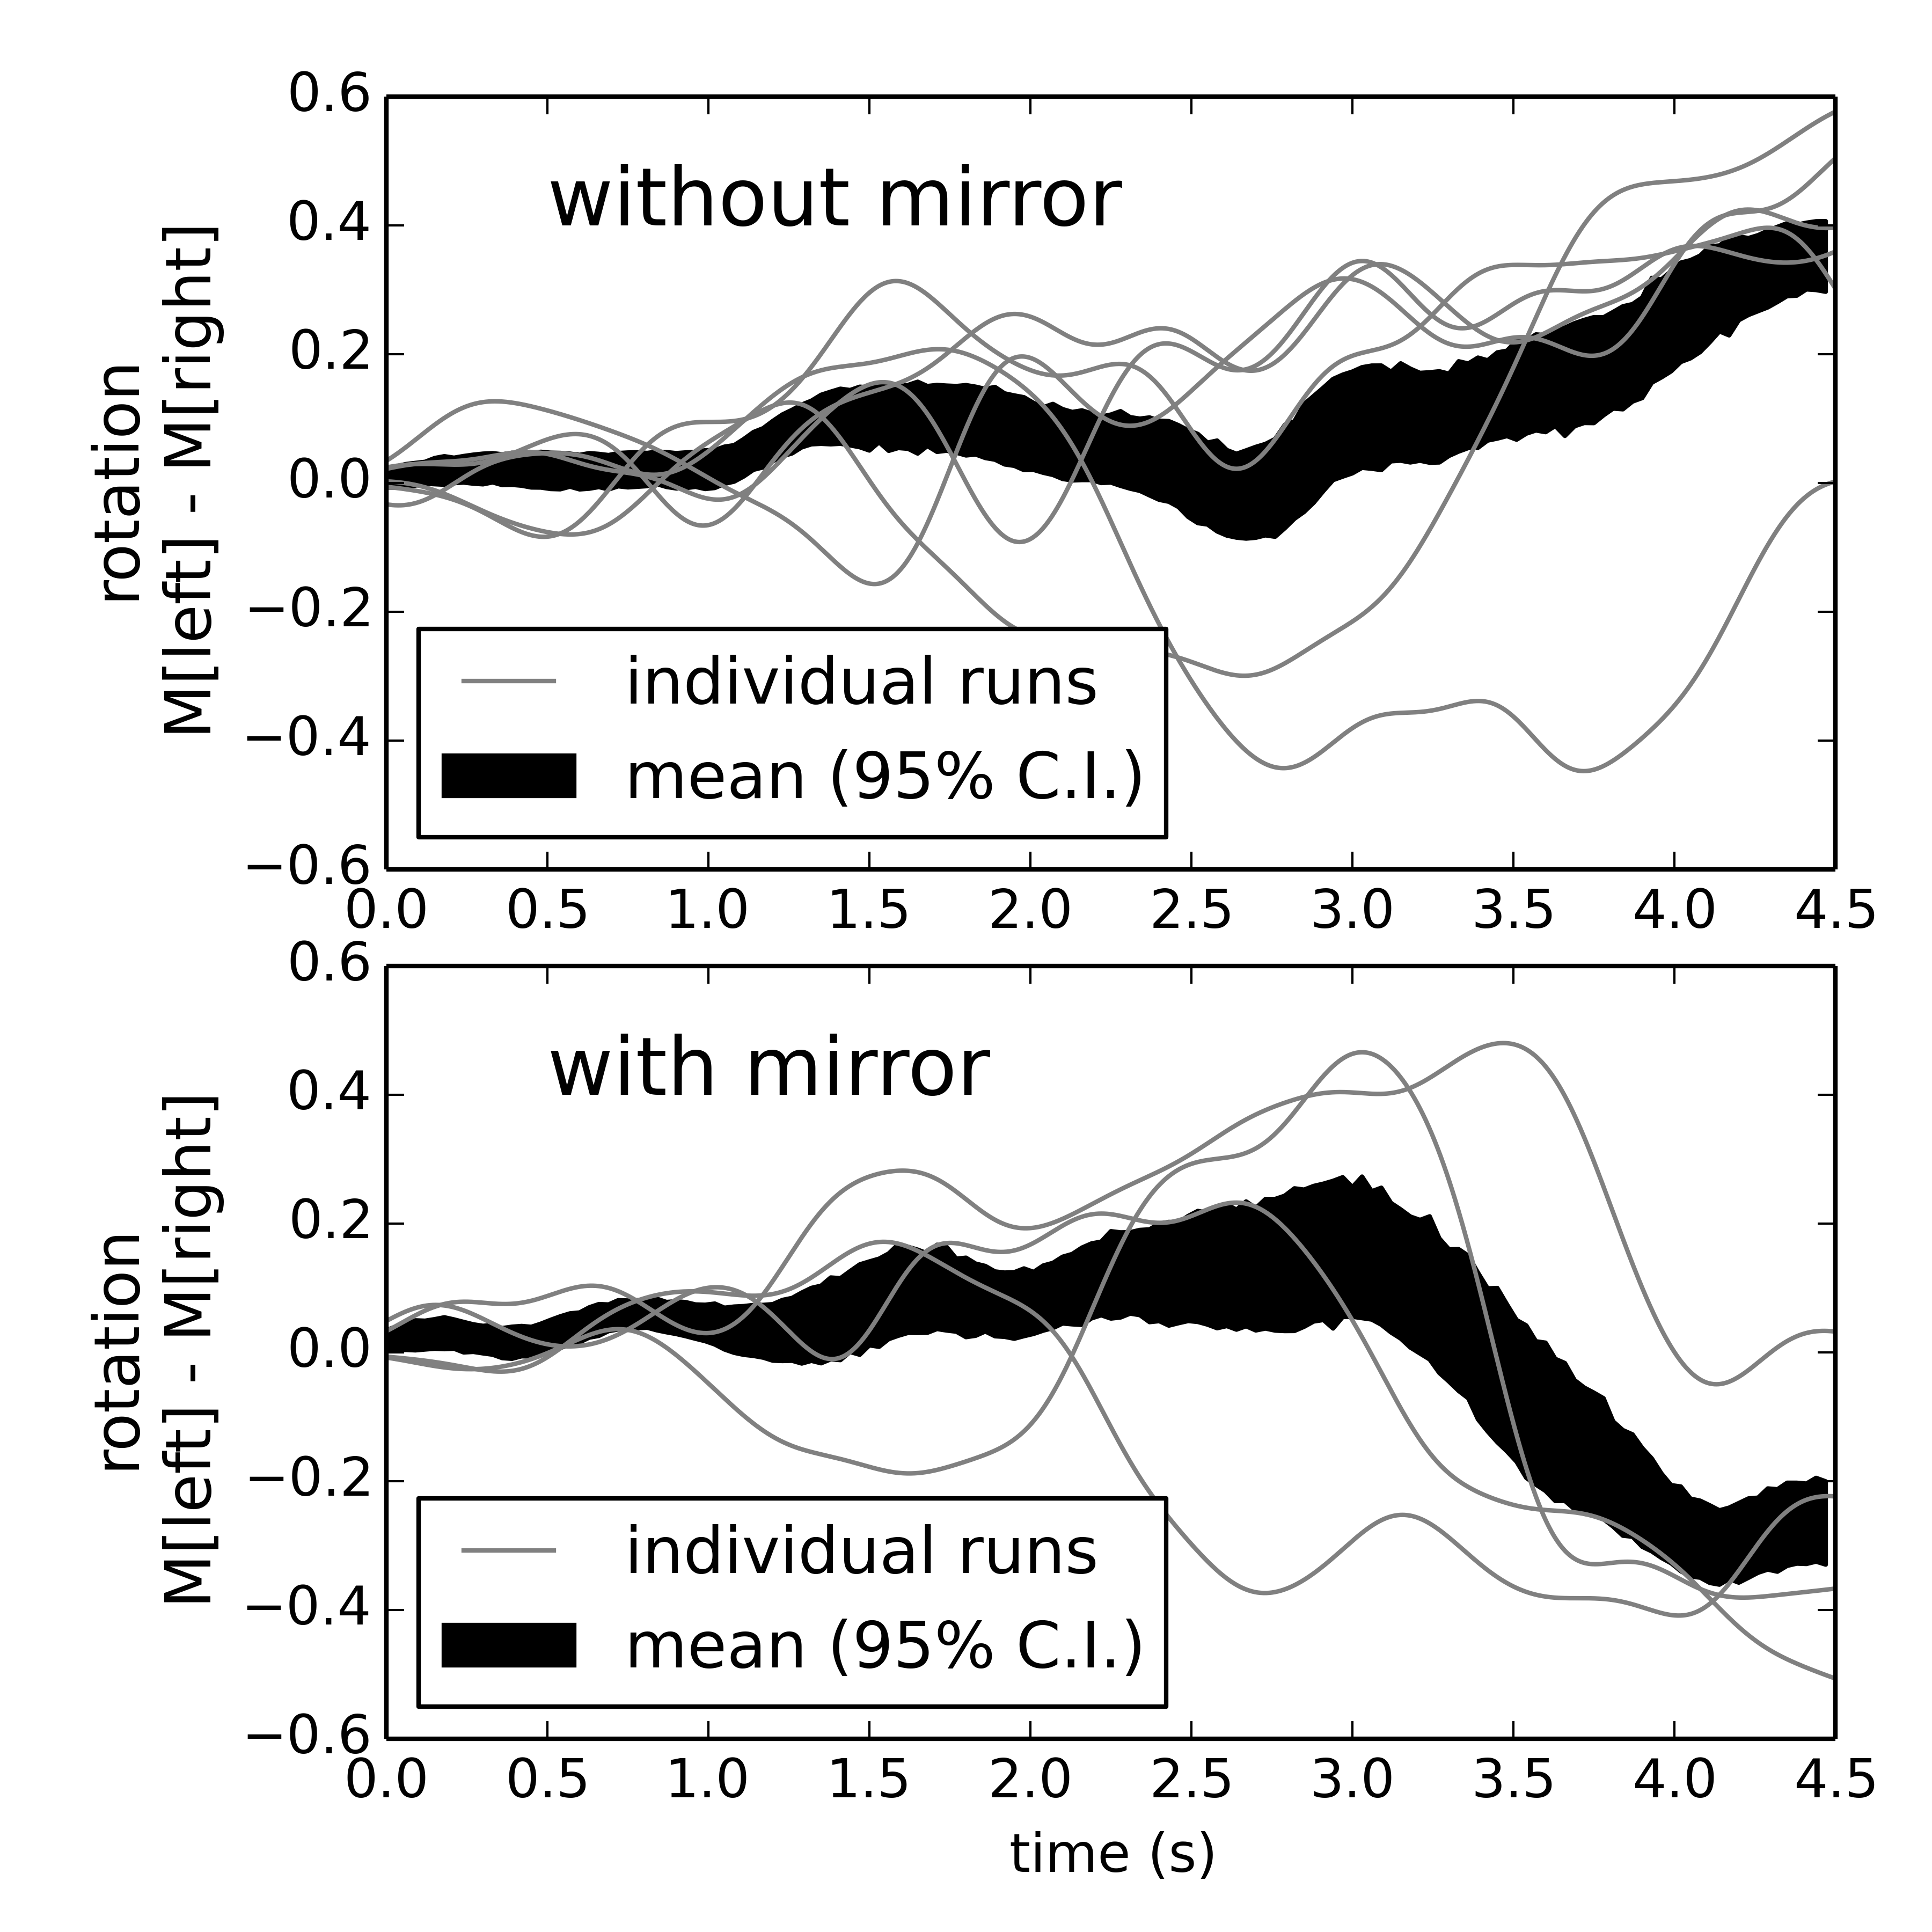
\includegraphics[width=2.5in]{learn-mirror/learnmirror.png}
% where an .eps filename suffix will be assumed under latex, 
% and a .pdf suffix will be assumed for pdflatex; or what has been declared
% via \DeclareGraphicsExtensions.
\caption{Behavior after learning to turn right if there is a mirror, and otherwise turn left. The robot successfully identifies the correct situation and turns appropriately. Robot speed is not shown, but is similar to that depicted at the top of \figurename~\ref{React}}
\label{Right}
\end{figure}

\section{Discussion}
The algorithm described in this paper is a general-purpose approach to
implementing mobile robot behaviours, 
making use of massively parallel low-power neuromorphic computing hardware. 
The basic algorithm is as follows:

\begin{itemize}
\item define a set of basic actions (e.g. driving forward, turning left)
\item define functions for how strong each action should be done, given the
current sensory state (e.g. drive forward if there is no obstacle ahead)
\item generate a neural network that approximates these functions
\item use the neural network to drive the robot and record the neural activity
\item identify a set of positive examples where the robot has accidentally
performed whatever other task is desired (e.g. turning towards a target object)
\item retrain the neural connections between the sensory neurons and the
action strengths so as to approximate the data gathered during the positive
examples
\end{itemize}

Using this approach, we have shown that we can take a network that
implements extremely simple manually specified reactive rules, and have
it learn by example to perform more complex functions.  This method
makes use of the power-efficiency of neuromorphic hardware, where large
numbers of neurons and connections can be used to efficiently
approximate complex functions.

In the case of the system learning to change its behavior based on the 
presence of a reflective mirror surface, the system was able to map the 
complex sensory stimuli to a particular motor action.  In particular, it
was able to make use of whatever sensory discrimination is available via
the mirror (or lack of a mirror).  It is important to note that this sensory 
stimulus did not initially impact the robot's behavior in any way. It was 
only through the process of learning, i.e. using hindsight examples of desired 
behavior and building a new set of connections that approximate required 
behavior that triggered changes in movement.  This was done by building neural
connections that replicate behaviour that the robot previously did accidentally.

A vital topic of future work is to characterize the variety of different
learned tasks that are amenable to this method.  In general, the NEF shows
that the accuracy of the learned connections are dependent on the complexity
of the function to be learned (in this case the mapping from sensor states to
action choices) and the number of neurons.  As we explore different tasks,
we will also need to explore different combinations of sensor systems and
the pre-processing on this data.  

This approach of using sensory experience to learn neural connections
that attempt to cause the same actions to occur in response to similar
sensory stimuli is novel, but we have performed previous work \cite{conradt2014trainable}
with a somewhat similar learning method. In that case, we did not have an 
initial reflexive control system, and we did not find particular examples of 
desired behavior. Instead, we put the robot temporarily under manual control 
and used the behavior generated by the person performing the manual control 
to train the connections between sensory neurons and motor neurons.  In other
words, rather than allowing the robot to randomly explore its environment and
choose actions based on a manually created reflexive control system, we had
a user manually set the motor outputs using a remote control.  As in this work
presented here, we then trained neural connections that would approximate that
manual control.  

In that earlier work, learning required direct training examples, rather than 
simply labelling particular actions as positive example of desired behavior 
after they occur.  Indeed, this means that the work presented here could be 
thought of as reinforcement learning, while the previous work would be purely 
supervised learning. Of course, a hybrid approach could be pursued. 

Finally, it should be noted that we are only training based on positive 
examples (i.e. situations where the robot behaved as desired). In future work,
we plan to augment this approach with explicit punishment for situations where 
the robot performs a non-desired behavior. Interestingly, adding this capability
is not straight-forward in this case.  Indeed, there is significant biological 
evidence that positive (reward), and negative (punishment) systems are separate 
in the brain [TODO: reference]. That is, they are not simply the opposite of 
each other –-- rather they are significantly different processes that interact. 
This interaction is still to be explored. One step towards this is a model
of fear conditioning \cite{kolbeck2013fear}, which would fit well with this framework.


% use section* for acknowledgement
\section*{Acknowledgement}

The Telluride Neuromorphic Cognition Workshop 2011. 

% trigger a \newpage just before the given reference
% number - used to balance the columns on the last page
% adjust value as needed - may need to be readjusted if
% the document is modified later
%\IEEEtriggeratref{8}
% The "triggered" command can be changed if desired:
%\IEEEtriggercmd{\enlargethispage{-5in}}

% references section
\bibliographystyle{IEEEtran}
% argument is your BibTeX string definitions and bibliography database(s)
\bibliography{refs}

\end{document}


